% ============================================================
% FIGURE 04: PERFORMANCE CHART (SUCCESS RATE)
% File: figure-04-performance-chart.tex
% Section: §5.1 Main Results
% Description: Comparison of Success Rate across dataset tiers.
% ============================================================

\begin{figure*}[htbp]
  \centering
  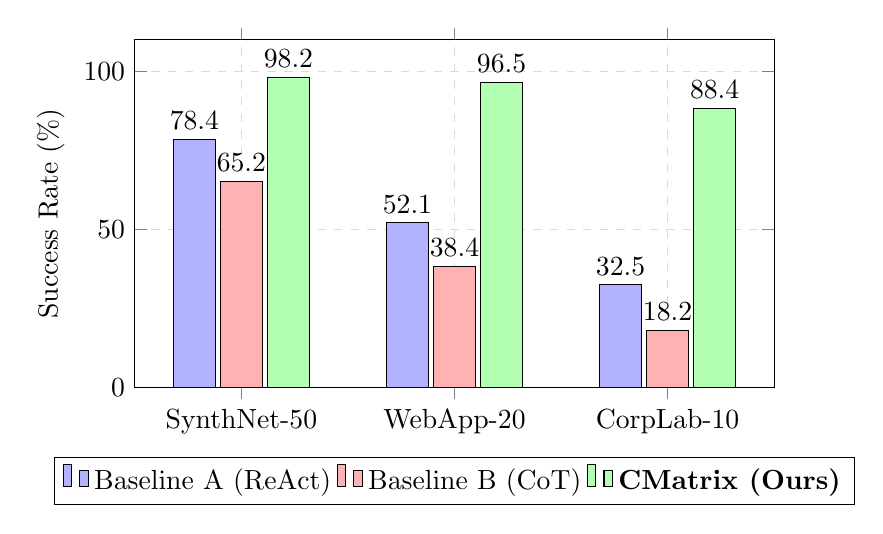
\begin{tikzpicture}
    \begin{axis}[
      ybar,
      enlarge x limits=0.25,
      legend style={at={(0.5,-0.2)}, anchor=north, legend columns=-1},
      ylabel={Success Rate (\%)},
      symbolic x coords={SynthNet-50, WebApp-20, CorpLab-10},
      xtick=data,
      nodes near coords,
      nodes near coords align={vertical},
      ymin=0, ymax=110,
      width=0.8\textwidth,
      height=6cm,
      bar width=15pt,
      grid=major,
      grid style={dashed, gray!30}
    ]
      % Baseline A (ReAct)
      \addplot[fill=blue!30] coordinates {(SynthNet-50, 78.4) (WebApp-20, 52.1) (CorpLab-10, 32.5)};
      % Baseline B (CoT)
      \addplot[fill=red!30] coordinates {(SynthNet-50, 65.2) (WebApp-20, 38.4) (CorpLab-10, 18.2)};
      % CMatrix (Full)
      \addplot[fill=green!30] coordinates {(SynthNet-50, 98.2) (WebApp-20, 96.5) (CorpLab-10, 88.4)};

      \legend{Baseline A (ReAct), Baseline B (CoT), \textbf{CMatrix (Ours)}}
    \end{axis}
  \end{tikzpicture}
  \caption{Task Success Rate across complexity tiers. CMatrix maintains high performance even as task complexity increases, significantly outperforming standard ReAct and CoT baselines in enterprise-scale environments.}
  \label{fig:performance-chart}
\end{figure*}
